\begin{naloga}{Bašić, Gajser}{Izpit OR 4.9.2012}
\begin{vprasanje}
Minolovec je stara Microsoftova računalniška igrica.
Dano je minsko polje v obliki kariraste mreže dimenzij $n \times m$,
v katerem se nahaja $p$ min.
Slika~\fig predstavlja delno odprto minsko polje, ki vsebuje $p = 40$ min.

V vsaki nedokončani igri je neka celica bodisi odprta bodisi zaprta.
V nekaterih zaprtih celicah se nahajajo mine.
V odprtih celicah so številke od $0$ do $8$
(številke 0 na sliki~\fig niso prikazane), ki povedo,
koliko min se nahaja v okolici te celice (tj., na sosednjih $8$ celicah).
Za razliko od Minolovca na računalniku lahko pri nas
tudi celica s številom $0$ meji na zaprto celico.

Delno odprto minsko polje (levo) ima pri $p = 7$ več možnih rešitev.
Dve sta prikazani na desni strani:
\begin{center}
\begin{tabular}{|p{0.2cm}|p{0.2cm}|p{0.2cm}|p{0.2cm}|p{0.2cm}|p{0.2cm}|p{0.2cm}|p{0.2cm}|p{0.2cm}|p{0.2cm}|p{0.2cm}|p{0.2cm}|p{0.2cm}|p{0.2cm}|p{0.2cm}|p{0.2cm}|p{0.2cm}|}
\cline{1-5} \cline{7-11} \cline{13-17}
&&&&& \qquad\qquad &
\bomb & \bomb & \bomb & \bomb && \qquad\qquad &
\bomb & \bomb & \bomb && \bomb \\
\cline{1-5} \cline{7-11} \cline{13-17}
2 & 3 & 4 &&&& 2 & 3 & 4 & \bomb &&& 2 & 3 & 4 & \bomb & \\
\cline{1-5} \cline{7-11} \cline{13-17}
0 & 0 & 2 &&&& 0 & 0 & 2 && \bomb && 0 & 0 & 2 & \bomb & \\
\cline{1-5} \cline{7-11} \cline{13-17}
0 & 0 & 1 &&&& 0 & 0 & 1 & \bomb &&& 0 & 0 & 1 && \bomb  \\
\cline{1-5} \cline{7-11} \cline{13-17}
\end{tabular}
\end{center}
Naslednje delno odprto minsko polje pa ni veljavno (ne glede na $p$):
\begin{center}
\begin{tabular}{|p{0.2cm}|p{0.2cm}|p{0.2cm}|p{0.2cm}|}
\hline
&&& \\ \hline
2 & 2 & 2 & \\ \hline
0 & 0 & 2 & \\ \hline
\end{tabular}
\end{center}

\begin{enumerate}[(a)]
\item Opiši celoštevilski linearni program, ki bo povedal,
ali je neko tako delno odprto minsko polje veljavno,
tj., ali je možno $p$ min postaviti na polje tako,
da bo v okolici vsake odprte celice ustrezno število min.

\item Ali bi lahko s pomočjo celoštevilskega linearnega programa ugotovil,
kolikšno je največje možno število min pri nekem delno odprtem polju?
\namig{morda zadošča, če malenkost popraviš program iz prejšnje točke.}

\item Kako bi s pomočjo zgornjega celoštevilskega linearnega programa
poiskal celice, ki nujno vsebujejo mino
(tj., pri vseh možnih rešitvah se v tistih celicah nahajajo mine)?
\end{enumerate}
Pri pisanju celoštevilskih linearnih programov si lahko pomagaš z oznakami:
\begin{itemize}
\item ${\mathcal O}$: množica vseh odprtih celic,
\item ${\mathcal Z}$: množica vseh zaprtih celic,
\item $N(s)$: množica sosedov celice $s$.
\end{itemize}

\begin{slika}
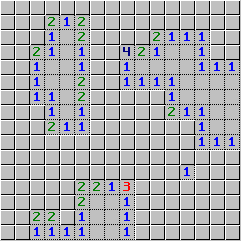
\includegraphics[width=0.5\textwidth]{slike/minolovec.png}
\podnaslov{Primer delno odprtega polja}
\end{slika}
\end{vprasanje}

\begin{odgovor}
Za vsako odprto celico $s \in {\mathcal O}$
naj $a_s$ označuje številko v celici $s$,
tj., število min v celicah iz množice $N(s)$.
Za vsako zaprto celico $t \in {\mathcal Z}$ bomo uvedli spremenljivko $x_t$,
katere vrednost interpretiramo kot
$$
x_t = \begin{cases}
1; & \text{v celici $t$ je mina, in} \\
0  & \text{sicer.}
\end{cases}
$$
Najprej zapišimo omejitve, ki jih bomo vseskozi upoštevali.
\begin{alignat*}{2}
\forall t \in {\mathcal Z}: &\ & 0 \le x_t &\le 1, \quad x_t \in \Z \\
\forall s \in {\mathcal O}: &\ &
\sum_{t \in N(s) \setminus {\mathcal O}} x_t &= a_s
\end{alignat*}

\begin{enumerate}[(a)]
\item Začetnim omejitvam dodamo še
$$
\sum_{t \in {\mathcal Z}} x_t = p .
$$
Zanima nas le obstoj dopustne rešitve,
zato ciljna funkcija ni pomembna.

\item Pri začetnih omejitvah uporabimo ciljno funkcijo
$$
\max \ \sum_{t \in {\mathcal Z}} x_t .
$$

\item Za vsako zaprto celico $r \in {\mathcal Z}$
poiščemo dopustno rešitev celoštevilskega linearnega programa
z začetnimi omejitvami
(in še omejitvijo iz točke (a), če poznamo skupno število min)
in ciljno funkcijo
$$
\min x_r .
$$
Če je celoštevilski linearni program dopusten
z vrednostjo ciljne funkcije enako $1$,
potem celica $r$ nujno vsebuje mino.
\end{enumerate}
\end{odgovor}
\end{naloga}
